%\section{「印刷する」機能}
本アプリにはカードリストから写真データや観光情報を取得することによって、1枚のリーフレットを作成する機能がある。トップ画面から印刷するボタンをタップするとリーフレットの写真選択画面に遷移する。リーフレットの写真選択画面は図6.6(a)に示す。写真の部分をタップするとリーフレット作成画面に遷移する。リーフレット作成画面に遷移した画面を図6.6(b)に示す。リーフレット作成画面ではリーフレットで使いたい画像をユーザに選んでもらう。ユーザがリーフレット作成画面で紹介された画像の中に使いたい画像があればこの写真を使うボタンをタップすることでリーフレットの写真選択画面に遷移し、選択した写真の画像が選んだ画像になる。このようにリーフレットに使いたい画像を7枚選んでもらう。7枚選んだ状態で右上の完了ボタンをタップすると印刷プレビュー画面に遷移する。7枚選んでいない状態で完了ボタンを押すと警告が発生し、すべて画像を選ぶように注意するようにした。印刷プレビュー画面は図6.6(c)に示す。そこでは実際にリーフレットの表側、裏側がどのように印刷されるのか確認することができる。もし、印刷されるリーフレットが気に入らなければ左上の戻るボタンを押すと写真選択画面に戻る。印刷されるリーフレットが気に入った場合は右上の完了ボタンを押すことでAirPrintの印刷画面に遷移する。AirPrintの印刷画面は図6.6(d)に示す。AirPrintの設定画面ではまず、接続するプリンタを 選択する。iPhoneとプリンタがWi-Fiに繋がっていれば、プリンタの欄に使用したいプリンタ名が表示されるので選択する。次に印刷する部数、印刷するページを片面にするのか両面にするのか選択した後右上のプリントボタンを押すとiPhoneからプリンタにデータが送信される。プリンタがWi-Fi経由でデータを受信するとリーフレットが印刷される.。
\begin{figure}[htbp]
  \begin{center}
    \begin{tabular}{c}

      % 1
      \begin{minipage}{0.33\hsize}
        \begin{center}
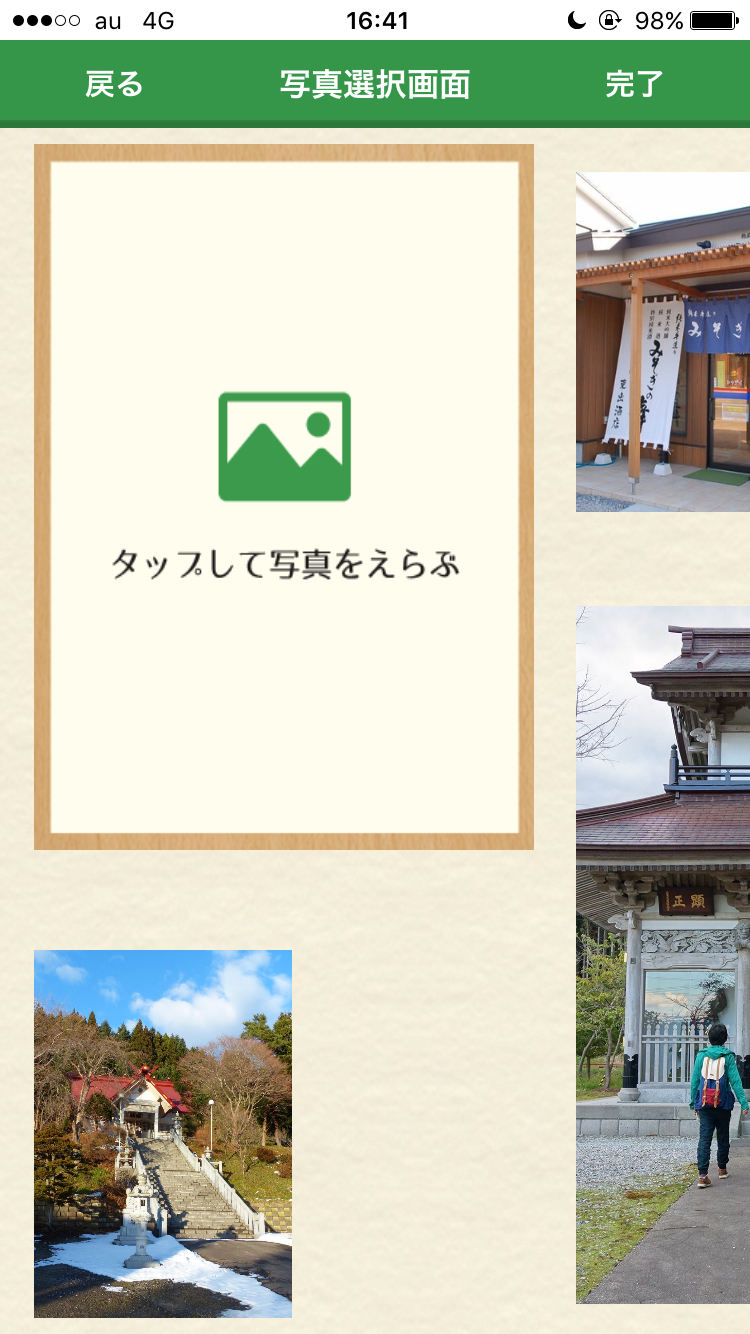
\includegraphics[width=4cm, bb=0 0 304 570]{kiko_print2.PNG}
          \hspace{1cm} (a)リーフレットの写真選択画面
        \end{center}
      \end{minipage}

      % 2
      \begin{minipage}{0.33\hsize}
        \begin{center}
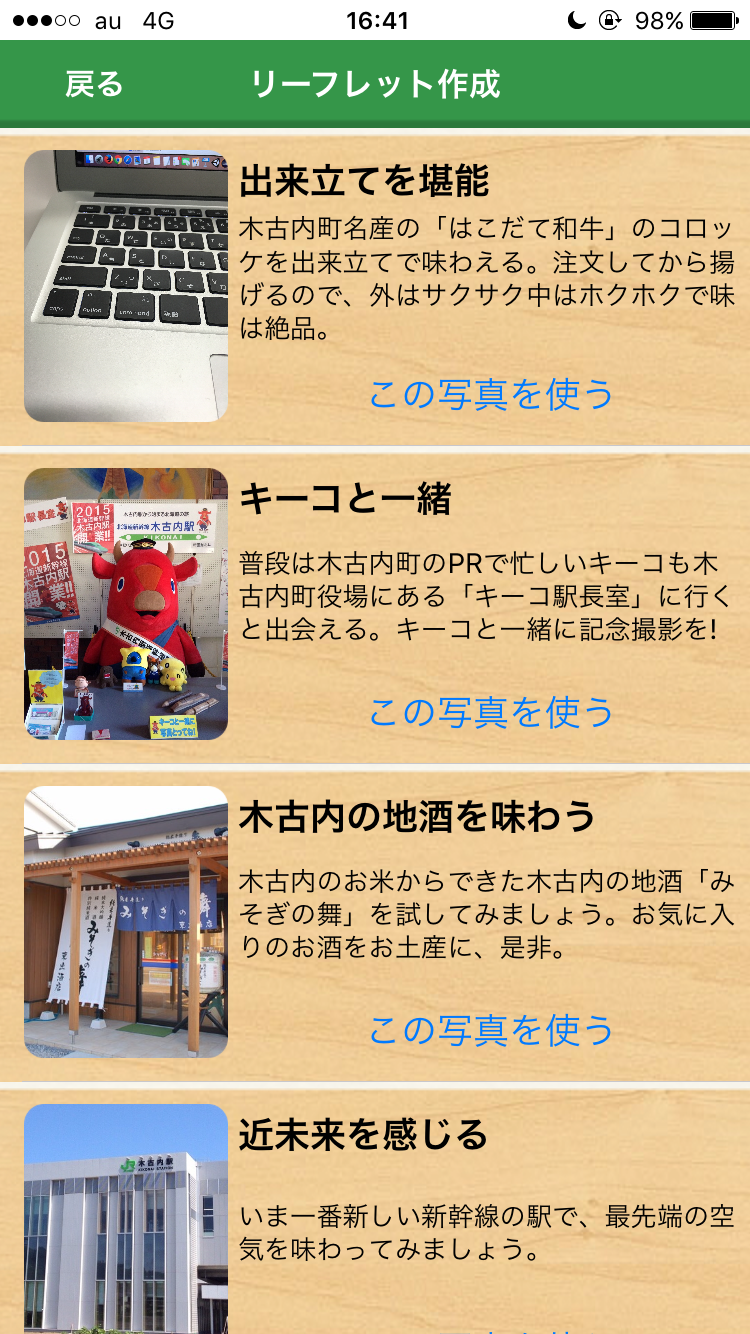
\includegraphics[width=4cm, bb=0 0 304 570]{kiko_print3.PNG}
          \hspace{1cm} (b)リーフレット作成画面
        \end{center}
      \end{minipage}
      
      \\
      
       % 3
      \begin{minipage}{0.33\hsize}
        \begin{center}
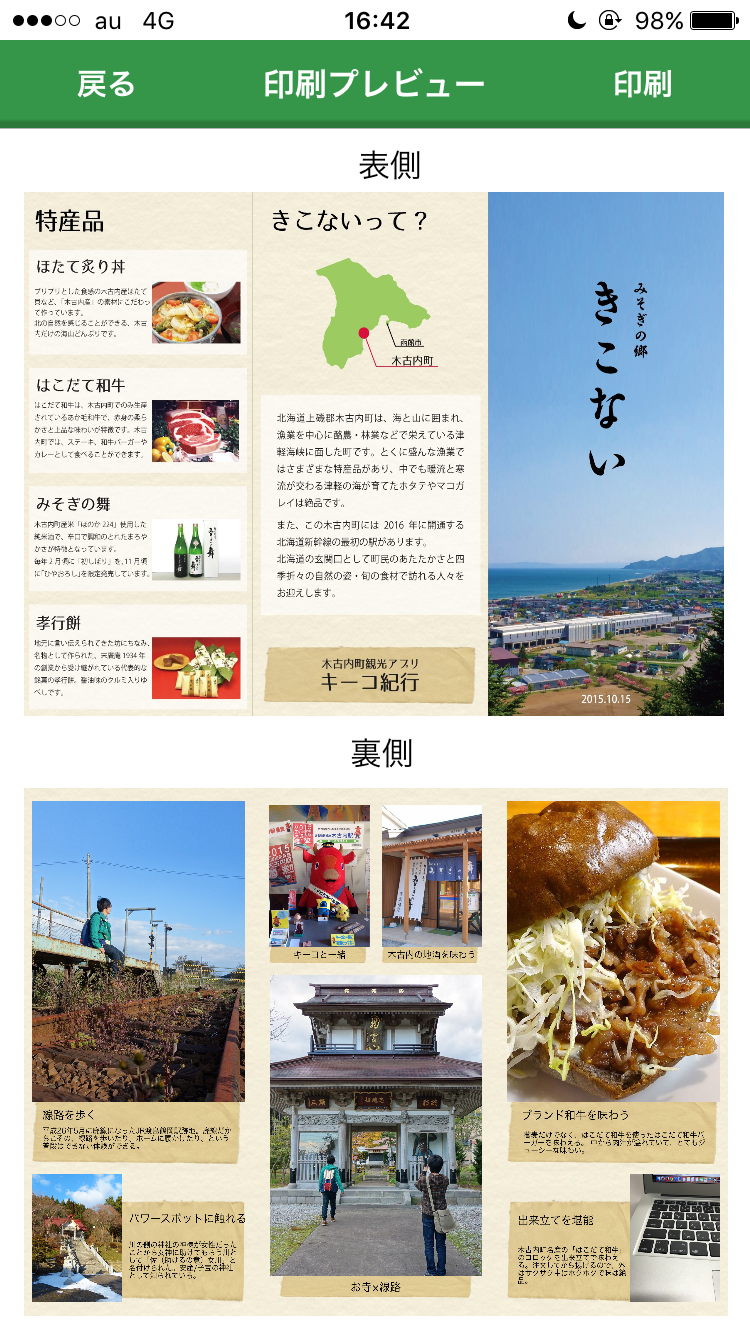
\includegraphics[width=4cm, bb=0 0 304 570]{kiko_print4.PNG}
          \hspace{1cm} (c)印刷プレビュー画面
        \end{center}
      \end{minipage}

      % 4
      \begin{minipage}{0.33\hsize}
        \begin{center}
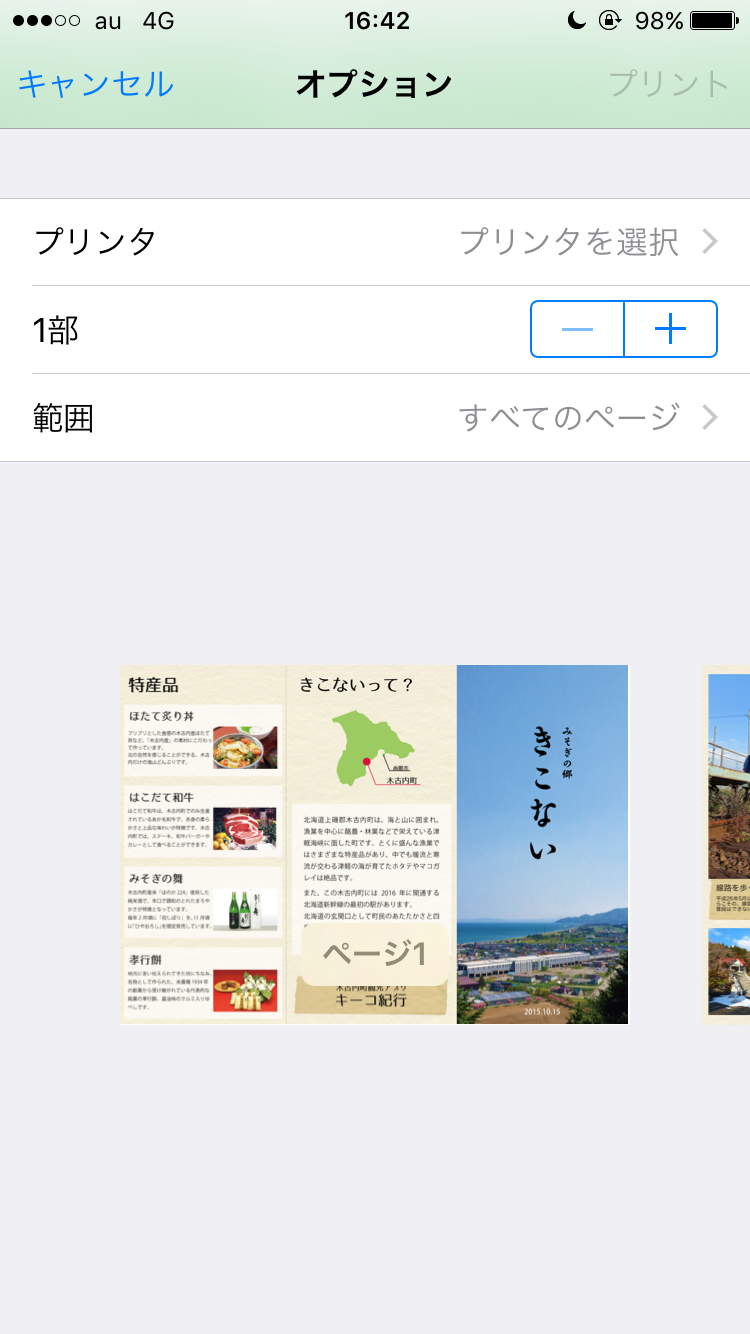
\includegraphics[width=4cm, bb=0 0 304 570]{kiko_print5.PNG}
          \hspace{1cm} (d)AirPrintの印刷画面
        \end{center}
      \end{minipage}
      

    \end{tabular}
    \caption{印刷機能の画面}
    \label{fig:lena}
  \end{center}
\end{figure}       

\bunseki{池田俊輝}